\documentclass[letterpaper,final,12pt,reqno]{amsart}

\usepackage[total={6.3in,9.2in},top=1.1in,left=1.1in]{geometry}

\usepackage{times,bm,bbm,empheq,fancyvrb,graphicx}
\usepackage[dvipsnames]{xcolor}
\usepackage{longtable}
\usepackage{booktabs}

\usepackage[within=section]{newfloat}

\usepackage{tikz}
\usetikzlibrary{decorations.pathreplacing}

\usepackage[kw]{pseudo}
\pseudoset{left-margin=15mm,topsep=5mm,idfont=\texttt}

% hyperref should be the last package we load
\usepackage[pdftex,
colorlinks=true,
plainpages=false, % only if colorlinks=true
linkcolor=blue,   % ...
citecolor=Red,    % ...
urlcolor=black    % ...
]{hyperref}

\renewcommand{\baselinestretch}{1.05}

\allowdisplaybreaks[1]  % allow display breaks in align environments, if they avoid major underfulls

\newtheoremstyle{claim}% name
  {5pt}% space above
  {5pt}% space below
  {\itshape}% body font
  {}% indent amount
  {\itshape}% theorem head font
  {.}% punctuation after theorem head
  {.5em}% space after theorem head
  {\thmname{#1}\thmnumber{ #2}\thmnote{ (#3)}}% theorem head spec
\theoremstyle{claim}
\newtheorem{theorem}{Theorem}
\newtheorem{lemma}{Lemma}

\newcommand{\eps}{\epsilon}
\newcommand{\RR}{\mathbb{R}}

\newcommand{\grad}{\nabla}
\newcommand{\Div}{\nabla\cdot}
\newcommand{\trace}{\operatorname{tr}}

\newcommand{\hbn}{\hat{\mathbf{n}}}

\newcommand{\bb}{\mathbf{b}}
\newcommand{\be}{\mathbf{e}}
\newcommand{\bbf}{\mathbf{f}}
\newcommand{\bg}{\mathbf{g}}
\newcommand{\bn}{\mathbf{n}}
\newcommand{\br}{\mathbf{r}}
\newcommand{\bu}{\mathbf{u}}
\newcommand{\bv}{\mathbf{v}}
\newcommand{\bw}{\mathbf{w}}
\newcommand{\bx}{\mathbf{x}}

\newcommand{\bF}{\mathbf{F}}
\newcommand{\bV}{\mathbf{V}}
\newcommand{\bX}{\mathbf{X}}

\newcommand{\bxi}{\bm{\xi}}

\newcommand{\bzero}{\bm{0}}

\newcommand{\rhoi}{\rho_{\text{i}}}

\newcommand{\ip}[2]{\left(#1,#2\right)}

\newcommand{\mR}{R^{\bm{\oplus}}}
\newcommand{\iR}{R^{\bullet}}

\newcommand{\pp}{{\text{p}}}
\newcommand{\qq}{{\text{q}}}
\newcommand{\rr}{{\text{r}}}

% norm |||x|||
\newcommand{\vertiii}[1]{{\left\vert\kern-0.25ex\left\vert\kern-0.25ex\left\vert #1 \right\vert\kern-0.25ex\right\vert\kern-0.25ex\right\vert}}

% numbering
\setcounter{tocdepth}{3}
\makeatletter
\def\l@subsection{\@tocline{2}{0pt}{4pc}{5pc}{}}
\makeatother

\numberwithin{equation}{section}
\numberwithin{figure}{section}
\numberwithin{table}{section}
\numberwithin{theorem}{section}

\DeclareFloatingEnvironment[name=Pseudocode]{pcode}

\begin{document}
\title[Multilevel computation of glacier geometry from Stokes dynamics]{Multilevel computation of glacier geometry \\ from Stokes dynamics}

\author{Ed Bueler}

\author{Lawrence Mitchell}

\begin{abstract} FIXME MCD for steady and evolving geometry with Glen-Stokes dynamics
\end{abstract}

\maketitle

%\tableofcontents

\thispagestyle{empty}
%\bigskip

\section{Introduction} \label{sec:intro}

FIXME MCD = multilevel constraint decomposition, a multigrid \cite{Trottenbergetal2001} method basically by \cite{Tai2003} for obstacle problems; see \cite{Bueler2022};  obstacle problem view first extended to Stokes by \cite{WirbelJarosch2020};  The computations in this paper use the Python FE library Firedrake \cite{Rathgeberetal2016}, which applies an embedded domain language \cite{Alnaesetal2014} to convert weak forms into discrete equations which are solved in parallel using the PETSc \cite{Balayetal2020} library.


\section{The steady ice geometry problem} \label{sec:stokesgeometry}

The standard model for determining the geometry of glaciers is based in part upon a dynamical description of ice flow, namely a shear-thinning version of the Stokes equations.  This Glen-Stokes ice-dynamics model can only determine the free-surface glacier geometry when it is combined with the surface kinematical equation (SKE) and a form of climate input, namely the rate of accumulation of snow or ablation, i.e.~melting and runoff.  In this section we state the strong form of this ``coupled'' glacier geometry model in the steady-state case, which we call the steady ice geometry problem (SIGP).  The emphasis here is on the complementarity-problem nature of the SIGP, often not explicit in the glaciers literature (e.g.~as observed by \cite{SchoofHewitt2013}).  We then define its weak form, noting along the way several unknown aspects of the theory.  Section \ref{sec:evolution} gives the straightfoward extension of the steady case to a time-discretized evolving-geometry model, the implicit ice geometry problem (IIGP).

The SIGP is defined on a fixed, bounded map-plane region $\Omega \subset \RR^d$ (Figure \ref{fig:stokesdomain}).  We denote the map-plane variables as $x$ when $d=1$ and $x,y$ when $d=2$.  On $\Omega$ we assume that a climatic mass balance (CMB) function $a(x,y)$ is defined at every point, whether or not ice is present at that location.  In ice-free areas this function could be described as the ``potential'' CMB, namely the annual balance of snow accumulation and potential melt if ice were present \cite{Cogleyetal2011}, e.g.~as computed by energy balance in a climate or weather model.  Here we assume $a$ has units of ice thickness per time, equivalently ice volume per area (in $\Omega$) per time, compatible with our assumption of constant ice density below.  Also we assume there is a bed elevation function $b(x,y)$ defined everywhere on $\Omega$, which determines the topography upon which the glacier sits.  The functions $a$ and $b$ are the data (inputs) of the SIGP.

\begin{figure}[t]
\begin{center}
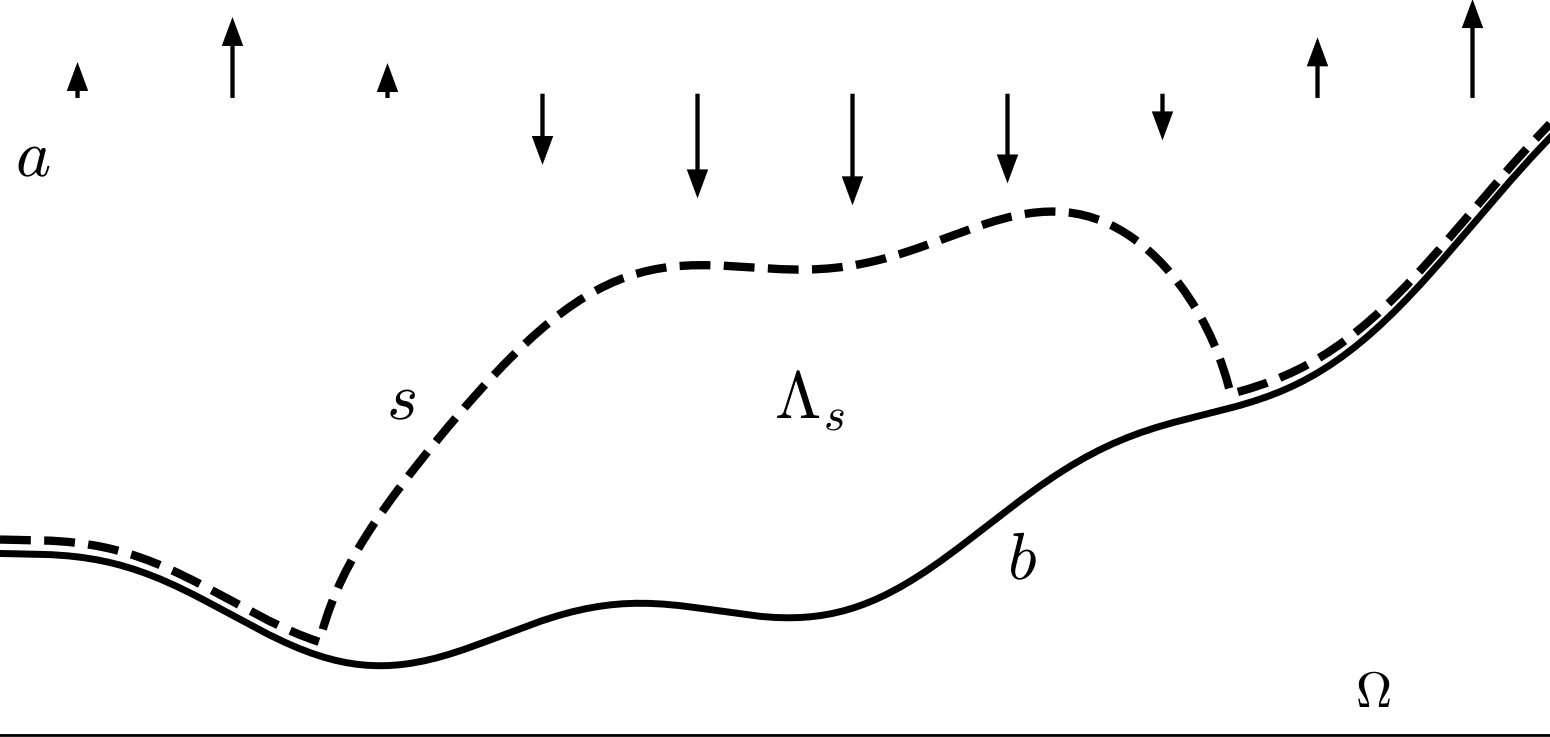
\includegraphics[width=0.75\textwidth]{genfigs/stokesdomain.pdf}
\end{center}
\caption{In the steady ice geometry problem (SIGP) the CMB $a$ (arrows; downward $=$ accumulation) and bed elevation $b$ (solid) are given on a fixed map-plane region $\Omega \subset \RR^d$.  The solution includes a surface elevation $s$ (dashed) on $\Omega$; note $s=b$ where ice-free.  The ice velocity $\bu$ and pressure $p$ are defined in the icy domain: $\Lambda_s = \{(x,y,z)\,:\,b(x,y) < z < s(x,y)\} \subset \RR^{d+1}$.}
\label{fig:stokesdomain}
\end{figure}

The Glen-Stokes dynamical model, the so-called stress balance, for ice only applies in the icy domain in $\RR^{d+1}$.  We make a strong, but common \cite[for example]{IsaacStadlerGhattas2015,Jouvetetal2008,Lengetal2012,WirbelJarosch2020} assumption this this icy domain has a well-defined upper surface elevation, a function $s(x,y)$.  That is, we assume there are \emph{no overhangs}, and that the under-side of the ice is in contact with the bed $b$.  We then define $s$ everywhere in $\Omega$ by extending with $s=b$ where ice is absent, thus $s\ge b$ applies on $\Omega$.  Note that $s$ is part of the model solution; it is not given data.

However, as a consequence of the no-overhangs assumption, the SIGP as described here is likely not to be well-posed because of an issue at the ice margin.  There may be no steady state because the fluid in the vicinity of a steep ice margin, especially on a steep bed feature, ``wants'' to generate an overhang, violating the assumption that $s$ is well-defined.  Furthermore the same concern applies to each time step of an evolving model; the model does not stop overhangs from appearing at the margin.  However, because overhangs are small features in large glaciers and ice sheets, essentially all modeling literature ignores this possibility and assumes well-defined surface elevation and thickness \cite{Jouvetetal2008,Lengetal2012,WirbelJarosch2020}.  An exception is \cite{PralongFunk2005}, who furthermore suggest a potentially well-posed continuum model, a nontrivial extension of the one here, in which serac and ice-cliff calving occurs via a damage variable and a stress-fracture failure criterion.  This extended model also explains one of our numerical boundary variants, a short, fixed-height cliff (Section \ref{sec:mcdstokes}), but overhangs are not allowed in any of our numerical constructions.

Based on the assumption of a well-defined upper surface, we define the (solution) extent of the ice as the open set
\begin{equation}
\Lambda_s = \{(x,y,z)\,|\,(x,y) \in \Omega \,\text{ and }\, b(x,y) < z < s(x,y)\}  \subset \RR^{d+1}, \label{eq:lambdas}
\end{equation}
where $z$ is vertically-upward.  (If $d=1$ then coordinates are ``$(x,z)$'' on $\Lambda_s$.)  The map-plane region $\Omega$ need not be connected or simply-connected, but even if so the solution set $\Lambda_s$ need not be.  However, $\Lambda_s$ has the topology of the product of an open subset of $\Omega$ and an interval, and we will approximate it using an extruded mesh (Section \ref{sec:fe}).

For a given geometry $\Lambda_s$, we model the ice as a very-viscous \cite{Acheson1990}, non-Newtonian fluid subject to Glen's shear-thinning flow law \cite{GreveBlatter2009}; see also \cite[Chapter 1]{FowlerNg2021}.  Allowing any Glen exponent $n\ge 1$, the equations inside $\Lambda_s$ are
\begin{align}
- \nabla \cdot \tau + \nabla p &= \rhoi \bg &&\text{\emph{stress balance}} \label{eq:forcebalance} \\
\nabla \cdot \bu &= 0 &&\text{\emph{incompressibility}} \label{eq:incompressible} \\
\tau &= B_n |D\bu|^{(1/n) - 1} D\bu  &&\text{\emph{flow law}} \label{eq:viscflowlaw}
\end{align}
The solution fields here are the velocity $\bu$, pressure $p$, and deviatoric stress $\tau$.  Equations \eqref{eq:forcebalance} and \eqref{eq:viscflowlaw} form the momentum conservation (stress balance) model, while \eqref{eq:incompressible} is an aspect of our mass conservation model.  As seen below, mass conservation on the free surface of $\Lambda_s$ requires an additional equation \eqref{eq:ske}.

Regarding tensors and their notation, recall that the (Cauchy) stress tensor $\sigma$ decomposes into the deviatoric part $\tau$ minus the pressure, i.e.~$\sigma = \tau - p\,I$, so equation \eqref{eq:forcebalance} simply says $-\Div \sigma = \rhoi \bg$.  The strain rate tensor $D\bu$ is the symmetric part of $\grad \bu$, $D\bu = \frac{1}{2} \left(\grad\bu + \grad\bu^\top\right)$, and the tensor norm used in \eqref{eq:viscflowlaw} satisfies $|D\bu|^2 = \frac{1}{2} (D\bu)_{ij} (D\bu)_{ij}$.  Because $D\bu$ is symmetric, and because it has trace zero by equation \eqref{eq:incompressible}, i.e.~$\trace(D\bu)=\nabla \cdot \bu = 0$, equation \eqref{eq:viscflowlaw} implies that $\tau$ is also symmetric with trace zero, thus that $p=-(d+1)^{-1} \trace \sigma$.

In computations we will use constants $n=3$, ice density $\rhoi=910 \,\text{kg}\,\text{m}^{-3}$ \cite{Huybrechtsetal1996}, and gravity $\bg=\left<0,0,-g\right>$, with $g=9.81\,\text{m}\,\text{s}^{-2}$.  The ice hardness $B_n$ is a constant because we assume isothermal conditions \cite{GreveBlatter2009}, with $B_3=6.8082\times 10^7\,\text{Pa}\,\text{s}^{1/3}$ \cite{Huybrechtsetal1996}.

For the $n=1$ (Newtonian) Stokes equations one would write \eqref{eq:viscflowlaw} as $\tau = 2\nu D\bu$ with viscosity $\nu>0$, but exponents $n>1$ imply an effective viscosity function of $|D\bu|$.  This would thus be singular in the limit of small strain rates, and so, motivated by the actual finite viscosity of glacier ice \cite{GreveBlatter2009}, we define the regularized effective viscosity
\begin{equation}
\nu_\eps = \frac{1}{2} B_n \left(|D\bu|^2 + \eps\, D_0^2\right)^{(\pp-2)/2}, \label{eq:regeffvisc}
\end{equation}
where $\pp=(1/n)+1$, with $\pp=4/3$ in computations.  The constant $D_0$ defines a strain-rate scale for glacier flow; $D_0 = 1 \,\text{a}^{-1}$ and $\eps = 10^{-4}$ are used here.  Also we eliminate $\tau$ and rewrite \eqref{eq:forcebalance} as $- \nabla \cdot \left(2 \nu_\eps\, D\bu\right) + \nabla p = \rhoi \mathbf{g}$, with a vector $p$-Laplacian as the leading-order term.

Our SIGP model uses dynamic boundary conditions for isolated, grounded, and non-sliding ice.  In addition to the already-stated assumption that the top and bottom boundaries of $\Lambda_s$ can be identified, we further assume these surfaces have well-defined tangents.  On the upper free surface we set a condition of zero applied stress,
\begin{equation}
\left(2 \nu_\eps D\bu - pI\right) \bn_s = \bzero  \qquad \qquad \text{\emph{top} } \overline{\partial} \Lambda_s \label{eq:topbc}
\end{equation}
where $\bn_s$ is any normal to $\overline{\partial} \Lambda_s$.  (Providing a nonzero atmospheric pressure at the surface is straightforward, but it has no important consequence.)  On the base we impose no slip:
\begin{equation}
\bu = \bzero  \qquad\qquad \text{\emph{base} } \underline{\partial} \Lambda_s. \label{eq:basebc}
\end{equation}

Note that the ice flow extends in the horizontal direction until a free boundary at the glacier margin is reached, and the surface gradient $\grad s$ may become singular there, but the top and bottom surfaces are assumed to meet at the margin (Figure \ref{fig:stokesdomain}).  An alternative geometry with a small cliff is also considered (Section \ref{sec:fe}).  Real glacier margins may indeed occur as fracture-generated cliffs \cite{PralongFunk2005}, but fracture processes are not modeled here.

The well-posedness of the above dynamics model, for fixed domain $\Lambda_s$, is proven by \cite{JouvetRappaz2011}, and the solution is a unique pair $(\bu,p)$ defined on $\Lambda_s$.  (The function spaces are identified below when stating the weak formulation.)  However, the simultaneous determination of $\Lambda_s$ and $(\bu,p)$ is the goal of the SIGP model.  Indeed, the above equations make no reference to the climate input function $a$, so we need another ``equation'', which we will see is actually an inequality.

\newcommand{\bus}{\bu|_s}

Noting that the surface elevation is already defined on all of $\Omega$, with $s=b$ off the ice, we also extend the surface normal $\bn_s$, thus we set
\begin{equation}
\bn_s = \left<-s_x,-s_y,1\right> \label{eq:surfacenormal}
\end{equation}
so that the (un-normalized) surface normal is specified almost everywhere on $\Omega$.  (By contrast, note that the dynamical boundary condition \eqref{eq:topbc} applies only on top of the ice.)  Furthermore we extend the surface value of the velocity to all of $\Omega$:
\begin{equation}
\bus(x,y) = \begin{cases} \bu(x,y,s(x,y)), & s(x,y) > b(x,y), \\
                     \bzero, & \text{elsewhere}. \end{cases} \label{eq:surfacevelocity}
\end{equation}
(The movement of the solid earth would determine $\bu|_b \ne 0$, thus $\bu|_s$ could be nonzero in ice-free areas, and a more-complete model could include this small effect.)

The steady-state surface kinematical equation (SKE) \cite[see equation (5.21)]{GreveBlatter2009} is the needed additional aspect of mass conservation:
\begin{equation}
\bus \cdot \bn_s + a = 0 \qquad \text{\emph{on the ice}}. \label{eq:ske}
\end{equation}
Note that $a(x,y)$ is the \emph{vertical} ice thickness added per time.  (Some references use a distinct quantity, namely the thickness added perpendicularly to the ice surface \cite{GreveBlatter2009}, which is significantly different if the gradient $\grad s$ is large.)

While the involved quantities are defined everywhere, kinematical balance \eqref{eq:ske} applies only \emph{on} the ice.  However $\bus \cdot \bn_s + a \le 0$ everywhere in $\Omega$ because $a$ is nonpositive in steady state in ice-free locations.  In fact, when combined with the constraint that $s\ge b$ everywhere on $\Omega$, SKE \eqref{eq:ske} is part of an infinite-dimensional nonlinear complementarity problem (NCP) \cite{Bueler2021conservation}.  Recall that an NCP on a finite-dimensional vector space $V=\RR^k$ combines the three statements $x\ge 0$, $F(x)\ge 0$, and $x F(x)=0$, where $F:V\to V$ \cite{FacchineiPang2003}.

We may now state the strong form of the SIGP as follows:
\begin{align}
s - b &\ge 0 && \text{on $\Omega$} \label{eq:strongform} \\
- \bu|_s \cdot \bn_s - a &\ge 0 && \text{\emph{same}} \notag \\
(s - b) (- \bu|_s \cdot \bn_s - a) &= 0 && \text{\emph{same}} \notag \\
- \nabla \cdot \left(2 \nu_\eps\, D\bu\right) + \nabla p - \rhoi \mathbf{g} &= \bzero && \text{on $\Lambda_s$} \notag \\
\nabla \cdot \bu &= 0 && \text{\emph{same}} \notag \\
\left(2 \nu_\eps D\bu - pI\right) \bn_s &= \bzero && \text{on $\overline{\partial} \Lambda_s$} \notag \\
\bu &= \bzero && \text{on $\underline{\partial} \Lambda_s$} \notag
\end{align}
(Definition \eqref{eq:regeffvisc} is also needed.)  The first three statements in \eqref{eq:strongform} form the NCP, but it is coupled to the dynamical boundary value problem formed by the last four statements.

The solution of \eqref{eq:strongform} is a triple of functions $s(x,y)$, $\bu(x,y,z)$, $p(x,y,z)$.  However, as the domain on which $\bu,p$ are defined is only known via the solution elevation $s$, \eqref{eq:strongform} is at best an incomplete description.  The weak form in the next section, using a $s\mapsto \bu|_s$ solution operator, will partially address this concern.  Whether in strong or weak form, this inequality-constrained system of PDEs has a largely-unknown theory regarding well-posedness and solution regularity.  However, certain well-posedness theory is known for the SIA version of this problem, with existence established by \cite{JouvetBueler2012}, and uniqueness in the flat bed case.

In Sections \ref{sec:fe}--\ref{sec:mcdstokes} we will construct and demonstrate a robust multilevel scheme for the numerical solution of the SIGP weak form (Section \ref{sec:weakido}).  As noted in Section \ref{sec:intro}, numerical solutions have traditionally applied explicit time-stepping, even when computing steady states, splitting the dynamics and the SKE into sub-steps and using truncation to address the NCP \cite[for example]{Jouvetetal2008,Lengetal2012}.  By contrast, the implicit time-stepping model in Section \ref{sec:evolution} avoids time-splitting and is unconditionally stable.


\section{Weak form and the ice dynamics operator} \label{sec:weakido}

The weak form of the fixed-geometry Glen-Stokes model for ice flow, which extends the linear Stokes weak form \cite{Elmanetal2014} to regularized power-law rheology, is relatively well-known \cite{IsaacStadlerGhattas2015,JouvetRappaz2011,Lengetal2012}, and we summarize it here.  Then we will address the weak form of the SIGP.

Denote by $W^{\text{k},\text{r}}$ the Sobolev space \cite{Evans2010} of functions with $k$ derivatives which are $r$th-power integrable.  Suppose for the moment that $\Lambda \subset \RR^{d+1}$ is a fixed, bounded domain on which we prescribe a Dirchlet condition $\bu=0$ on some positive-measure portion of the boundary, and otherwise suppose the boundary is stress-free (Neumann boundary).  Let $\pp=(1/n)+1$ as in \eqref{eq:regeffvisc}, and let $\qq=(1-\pp^{-1})^{-1}=n+1$ be the conjugate exponent; $\pp=4/3$ and $\qq = 4$ if $n=3$.  Let $W_0^{1,\pp}(\Lambda)^{d+1}$ be the space of velocity functions, zero along the Dirichlet boundary, and
\begin{equation}
\mathcal{M}_{\text{GS}} = W_0^{1,\pp}(\Lambda)^{d+1} \times L^\qq(\Lambda)  \label{eq:mixed}
\end{equation}
be the (mixed) space of admissible velocity and pressure pairs.  The Glen-Stokes weak form is the statement that $(\bu,p) \in \mathcal{M}_{\text{GS}}$ should satisfy
\begin{equation}
F_{\text{GS}}(\bu,p)[\bv,q] = \int_\Lambda 2 \nu_\eps D\bu : D\bv - p \Div\bv - (\Div\bu) q - \rhoi \bg \cdot \bv\,d\bx = 0 \label{eq:glenstokesweak}
\end{equation}
for all $(\bv,q) \in \mathcal{M}_{\text{GS}}$.

Jouvet and Rappaz \cite{JouvetRappaz2011} prove that this Glen-Stokes formulation is well-posed under the above assumptions if also the Neumann boundary is $C^1$.  In particular they show \eqref{eq:glenstokesweak} is equivalent to minimization of a convex and coercive functional over the divergence-free subspace, but also that there is a unique pressure $p\in L^\qq(\Lambda)$.

However, we seek to go beyond this dynamical problem on predetermined ice geometry.  We are interested in finding a triple $s,\bu,p$ which solves \eqref{eq:strongform}, or rather its weak form which we now propose.  Again suppose $\Omega \subset \RR^d$ is a fixed map-plane domain with $C^1$ boundary, and that the bed elevation $b$ is in $W^{1,\qq}(\Omega)$.  Because of the $C^1$ boundary, the Sobolev space $W^{1,\qq}(\Omega)$ supports a linear trace operator which defines $f|_{\partial \Omega}$ for $f \in W^{1,\qq}(\Omega)$ \cite[Section 5.5]{Evans2010}.  Let
\begin{equation}
\mathcal{K} = \{s \in W^{1,\qq}(\Omega) \,:\, s \ge b \, \text{ and } \, s\big|_{\partial\Omega} = b\big|_{\partial\Omega}\}  \label{eq:Kconstraintset}
\end{equation}
be the closed and convex set of admissible surface elevations of an isolated glacier or ice sheet.  However, it is not clear that the correct Sobolev space has been identified in \eqref{eq:Kconstraintset}, and in fact we must further suppose that
\begin{equation}
s\in \mathcal{K} \text{ defines an icy domain } \Lambda_s \text{ which has a $C^1$ free surface.} \label{eq:quixotic}
\end{equation}
Quixotic assumption \eqref{eq:quixotic} would follow from a sufficiently-strong regularity result for the theory of the current paper, which we cannot offer.  However, the existing theory of shallow ice sheet well-posedness \cite{JouvetBueler2012} includes a version of definition \eqref{eq:Kconstraintset},\footnote{In \cite{JouvetBueler2012} the $2\qq/(\qq-1)=8/3$ power of the ice thickness is in $W^{1,\qq}(\Omega)$.} and in that shallow theory $s$ solves an elliptic equation and is thus smooth, at least interior to the free boundary.

We may now define the ice dynamics operator (IDO), a map using the trace of the velocity solution to the Glen-Stokes problem above (Figure \ref{fig:idoaction}).  For each surface elevation function $s \in \mathcal{K}$ the IDO result $\Phi(s)$ is the normal component of the upper-surface trace of the unique velocity solution $\bu$ of \eqref{eq:glenstokesweak} over the icy domain $\Lambda_s$, but extended by zero to all of $\Omega$:
\begin{equation}
\Phi(s) = \begin{cases} \bu|_{\overline{\partial} \Lambda_s} \cdot \bn_s, & s > b, \\
                        0, & \text{otherwise}, \end{cases} \label{eq:ido}
\end{equation}
where $\bu|_{\overline{\partial} \Lambda_s}$ denotes a trace operator on $W^{1,\pp}(\Lambda_s)^{d+1}$; compare \eqref{eq:mixed}.  Note that the output $\Phi(s)$, a scalar function on $\Omega$, may jump or have other singularities at the glacier margin, but we will only need $\Phi(s)$ to be in the dual of $W^{1,\qq}(\Omega)$, thus permitting substantial irregularities.

\begin{figure}[t]
\begin{center}
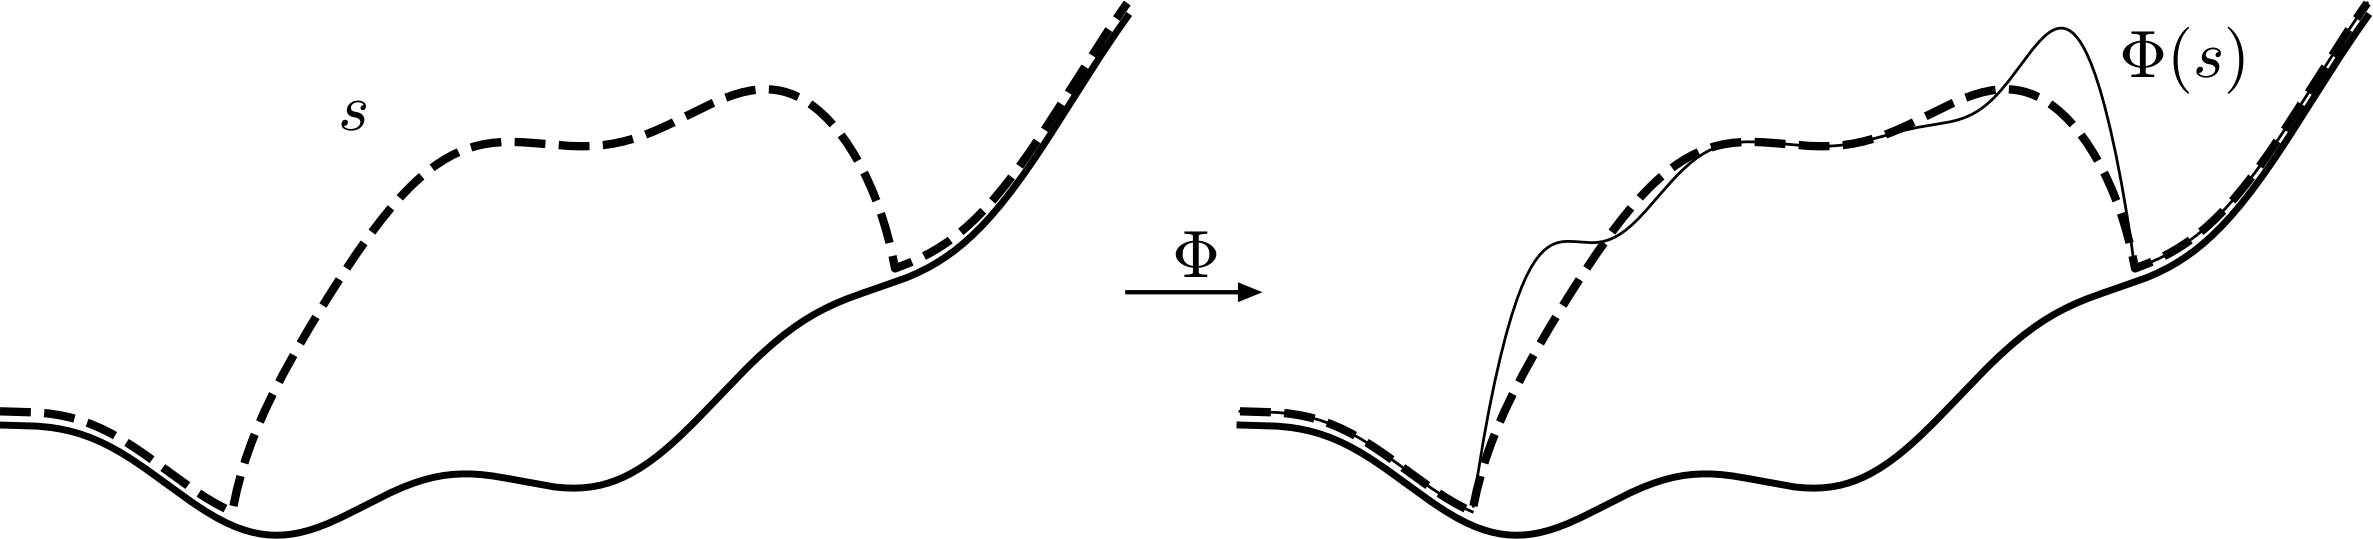
\includegraphics[width=\textwidth]{genfigs/idoaction.pdf}
\end{center}
\caption{The ice dynamics operator $\Phi$ maps the surface elevation $s$ (dashed) to the normal ice surface motion $\Phi(s)=\bu|_s \cdot \bn_s$; the thin line is $s+\Phi(s)$.  Both the input and output of $\Phi$ are defined on all of $\Omega$.}
\label{fig:idoaction}
\end{figure}

Using the IDO, and recalling that the CMB $a$ is defined on all of $\Omega$, we may immediately re-write the \eqref{eq:strongform} in a simpler strong form, namely an NCP with a hidden dynamical problem:
\begin{align}
s - b &\ge 0  \label{eq:idostrongform} \\
- \Phi(s) - a &\ge 0 \notag \\
(s - b) (- \Phi(s) - a) &= 0 \notag
\end{align}
Here the statements hold on all of $\Omega$ and the data $a,b$ are clear.  The solution is the ice surface $z=s(x,y)$, but $\bu,p$ are hidden variables within the evaluation of $\Phi(s)$.

For $s \in \mathcal{K}$ and $r \in W^{1,\qq}(\Omega)$ we next define a functional which is nonlinear in $s$:
\begin{equation}
F(s)[r] = - \ip{\Phi(s)}{r} = - \int_\Omega \Phi(s)\, r \,dx dy. \label{eq:sigpfunctional}
\end{equation}
One computes $F(s)[r]$ by defining the icy domain $\Lambda_s$ \eqref{eq:lambdas}, then solving the (weak form) Glen-Stokes problem \eqref{eq:glenstokesweak}, then evaluating the normal component of the surface trace of the velocity \eqref{eq:ido} to compute the IDO $\Phi(s)$, and then integrating the result against the test function $r$.  Implicit in \eqref{eq:sigpfunctional} is that $\Phi(s)$ has minimal regularity; it need only be in the dual space of $W^{1,\qq}(\Omega)$.

Finally, the SIGP weak form is the following variational inequality (VI) \cite{KinderlehrerStampacchia1980} which should determine $s\in\mathcal{K}$:
\begin{equation}
F(s)[r - s] \ge \ip{a}{r-s} \quad \text{for all $r \in \mathcal{K}$.}  \label{eq:sigpweakform}
\end{equation}
This VI has a shallow (SIA) analog, for which existence has been proven \cite{JouvetBueler2012}, but in that case the functional is an integral of powers of the thickness $s-b$ and the surface slope $\grad s$, thus locally-computable.  Here, by contrast, the computation of \eqref{eq:sigpfunctional} is non-local and expensive: to evaluate $F(s)[r]$ one must solve Glen-Stokes problem \eqref{eq:glenstokesweak} on the given $z=s(x,y)$ geometry.

Definition \eqref{eq:sigpfunctional} is a dual pairing of $F(s)$ and $r$, thus roughly an inner product.  VI \eqref{eq:sigpweakform} says that $s$ is located in $\mathcal{K}$, generically on $\partial\mathcal{K}$, at a place where $F(s)$ points directly into $\mathcal{K}$.  Specifically, in geometrical analogy, \eqref{eq:sigpweakform} says that the ``angle'' between $F(s)$ and an arbitrary vector $r-s$ pointing into $\mathcal{K}$ is at most $90^\circ$.

It is well-known that some VIs arise as inequality-constrained minimization problems \cite{GraeserKornhuber2009,KinderlehrerStampacchia1980}, but to the best of our knowledge VI \eqref{eq:sigpweakform} does \emph{not} arise in this way.  The general-bed, steady shallow (SIA) model is not a minimization, except in the flat-bed case \cite{JouvetBueler2012}.

The SIGP weak form \eqref{eq:sigpweakform} is coupled to \eqref{eq:glenstokesweak} through the definition of the IDO $\Phi$.  The problem therefore has three fundamental nonlinearities:
\renewcommand{\labelenumi}{(\emph{\roman{enumi}})}
\begin{enumerate}
\item the Glen power-law rheology,
\item the inequality constraint, and
\item the nonlinearity of free-surface flow reflected in the nonlinearity of the operator $\Phi$.
\end{enumerate}
Regarding (\emph{ii}), observe that even the classical obstacle problem for the linear Laplacian operator is nonlinear \cite{KinderlehrerStampacchia1980}.  Regarding (\emph{iii}), note that a free-surface flow for Newtonian (linear) rheology produces a nonlinear equation for the flow thickness, e.g.~as expressed in the kinematic wave equation \cite{Ockendonetal2003}.

To numerically solve \eqref{eq:sigpweakform} we will need the (Gateaux) derivative of $F$, which requires differentiating the $\Phi$ as well.  Suppose $s\in \mathcal{K}$, $\eps>0$, and $t \in W^{1,\qq}(\Omega)$ is such that $s+\eps t \in \mathcal{K}$.  (Both $s$ and $s+\eps t$ must be admissible glacier surface elevations.)  From \eqref{eq:sigpfunctional},
\begin{equation}
F'(s)[t,r] = \lim_{\eps\to 0^+} \frac{F(s+\eps t)[r] - F(s)[r]}{\eps} = - \int_\Omega \Phi'(s)[t]\, r \,dx dy \label{eq:sigpfunctionalderiv}
\end{equation}
where by definition
\begin{equation}
\Phi'(s)[t] = \lim_{\eps\to 0^+} \frac{\bu|_{s+\eps t} \cdot \bn_{s+\eps t} - \bus \cdot \bn_s}{\eps}. \label{eq:idoderiv}
\end{equation}
In \eqref{eq:idoderiv} note that the normal vectors and surface velocities are extended to the whole of $\Omega$; see \eqref{eq:surfacevelocity}.  We will assume that $\Phi'(s)[t]$ is in the dual space of $W^{1,\qq}(\Omega)$ so that \eqref{eq:sigpfunctionalderiv} is finite.  Observe that $F'$ is straightforward to compute from $\Phi'$.

Note $F'(s)[t,r]$ and $\Phi'(s)[t]$ are one-sided directional derivatives in the sense that $s+\eps t$ must be admissible, i.e.~$s+\eps t\ge b$, for all sufficiently-small $\eps>0$, and this clearly requires $t\ge 0$ on the (active) set where $s=b$.  However, to simplify our considerations we define an $s$-independent set
\begin{equation}
\mathcal{D}_+ = \{t \in W^{1,\qq}(\Omega) \,:\, t(x,y) \ge 0\}, \label{eq:infdefectset}
\end{equation}
so $\Phi'(s)[t]$ is well-defined on inputs $(s,t) \in \mathcal{K} \times \mathcal{D}_+$ and $F'(s)[t,r]$ is well-defined for $(s,t,r) \in \mathcal{K} \times \mathcal{D}_+ \times W^{1,\qq}(\Omega)$.

We will approximate the true derivative $\Phi'(s)[t]$ by the difference quotient in \eqref{eq:idoderiv}, but only in the situation where $t \in \mathcal{D}_+$ has small support.  (It will be a finite element basis function; see the next section.)  For this it is relevant to say more about the difference, as it depends on whether the point is in the support of $t$ or not:
\begin{align}
\bu|_{s+\eps t} \cdot \bn_{s+\eps t} - \bus \cdot \bn_s &= \left(\bu|_{s+\eps t} \cdot \bn_{s+\eps t} - \bus \cdot \bn_{s+\eps t}\right) + \left(\bus \cdot \bn_{s+\eps t} - \bus \cdot \bn_s\right) \label{eq:differencecases} \\
    &= \begin{cases}
           (\bu|_{s+\eps t} - \bus) \cdot \bn_{s+\eps t} + \eps\, \bus \cdot \left<t_x,t_y,0\right>, & s > b \\
           \bu|_{s+\eps t} \cdot \bn_{s+\eps t}, & s=b \text{ and } t > 0 \\
           0, & s=b \text{ and } t = 0
                 \end{cases} \notag
\end{align}
Thus a necessary condition for differentiability of $\Phi$ is that $\bu|_{s+\eps t} \cdot \bn_{s+\eps t} = o(\eps)$ on the ice-free area $s=b$.  In physical terms this means that the dynamical part of the SKE vanishes for small ice masses on bare ground, and it is reasonable to suppose this is so if the ice cannot slide.

In the next three sections we will construct an iterative, multilevel finite element solver for SIGP weak form \eqref{eq:sigpweakform}.  When we approximate the true derivative $\Phi'(s)[t]$ by a difference quotient, a significant issue arises because two Glen-Stokes solutions over the ice domains $\Lambda_{s+\eps t}$ and $\Lambda_s$ are seemingly required.  While this would imply a very large numbers of expensive dynamical solves, in Section \ref{sec:smoothers} we propose a less-expensive approximation.


\section{Finite element discretization} \label{sec:fe}

Assume $\Omega \subset \RR^d$ is polygonal and suppose $\mathcal{T}$ is a triangulation of $\Omega$.  (If $d=1$ then instead $\mathcal{T}$ denotes an interval decomposition of $\Omega$.)  Based on low expected regularity at the ice margin, we will represent surface elevations $s\in \mathcal{K}$ using the $P_1$ finite element (FE) space
\begin{equation}
\mathcal{V}^h = \{s \in C^0(\Omega) : s|_T \text{ is linear if } T \in \mathcal{T}\} \subset W^{1,\qq}(\Omega).
\end{equation}
Note \cite{JouvetBueler2012} makes the same FE choice for the corresponding shallow problem.

Let $b^h \in \mathcal{V}^h$ be the discretized bed elevation, e.g.~the $\mathcal{V}^h$ interpolant of $b$.  From $b^h$ we define the closed and convex admissible subset of $\mathcal{V}^h$:
\begin{equation}
\mathcal{K}^h = \{r^h \in \mathcal{V}^h \,:\, r^h \ge b^h \text{ and } r^h|_{\partial\Omega} = b^h|_{\partial\Omega}\}.  \label{eq:feK}
\end{equation}
For $s^h\in \mathcal{K}^h$ we also define the numerical icy domain as in \eqref{eq:lambdas}:
\begin{equation}
\Lambda_{s^h} = \{(x,y,z)\,:\,b^h(x,y) < z < s^h(x,y)\} \subset \RR^{d+1}.  \label{eq:felambdas}
\end{equation}
Also, a triangle (interval) $T\in\mathcal{T}$ is said to be ice-free in the $s^h$ geometry if $s^h=b^h$ at every vertex of $T$, and icy otherwise.

Given $s^h$ and $b^h$ from $\mathcal{V}^h$, we construct a Firedrake extruded mesh \cite{McRaeetal2016} to decompose $\Lambda_{s^h}$.  If $d=2$ then the extruded mesh consists of triangular prisms, while if $d=1$ it has quadrilateral elements.  The extruded mesh construction starts from the triangulation $\mathcal{T}$ of $\Omega \subset \RR^d$, now called the ``base mesh''.  As shown in Figure \ref{fig:extruded}, each icy $T$ generates a column of $m_z \ge 1$ prism (quadrilateral) elements in the extruded mesh.  However, ice-free $T$ have no extruded mesh elements at all; these columns are empty.

\begin{figure}[t]
\begin{center}
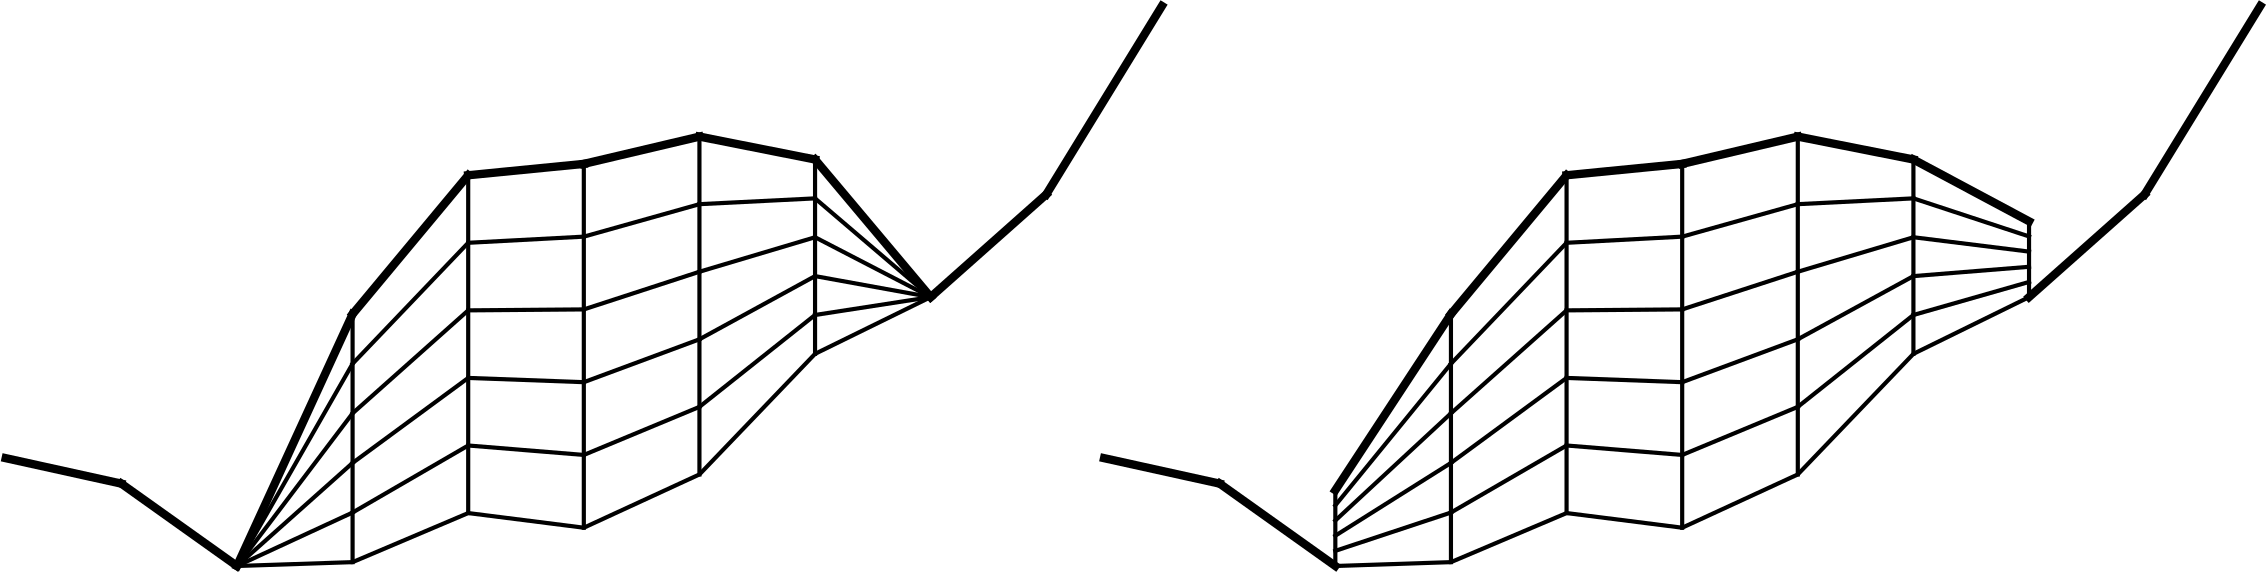
\includegraphics[width=\textwidth]{genfigs/extruded.pdf}
\end{center}
\caption{We compute $\Phi^h(s^h)$ by solving \eqref{eq:glenstokesweak} on an extruded mesh with $m_z$ layers.  In the ``pinched'' extrusion (left), the trace of $\bu^h$ is evaluated on the graph of $s^h$ (bold); see \eqref{eq:ido}.  In the ``cliffs'' extrusion (right) all elements have a minimum thickness and the trace evaluation (bold) may occur above $s^h$ (dotted).}
\label{fig:extruded}
\end{figure}

We will compare two extrusion modes.  In the ``pinched'' extrusion the elements cover $\Lambda_{s^h}$ exactly, prism (quadilateral) elements at the ice margin degenerate; such elements have empty facets.  In the alternate ``cliffs'' extrusion, each element over an icy $T$ is nondegenerate.  Specifically, if $H_{\text{min}} > 0$ is the minimum total thickness, with $H_{\text{min}} = 20$ meters in experiments, then each prism (quadilateral) element has minimum thickness $H_{\text{min}}/m_z$.  In this extrusion, a stress-free condition is applied on the cliffs  in the Glen-Stokes problem \eqref{eq:glenstokesweak}; they are treated the same way as the top surface.

Let $\Phi^h:\mathcal{K}^h \to (\mathcal{V}^h)'$ be the FE approximation of the IDO $\Phi$.  By definition $\Phi^h(s^h)$ is the normal component of the numerical surface velocity after solving the Glen-Stokes equation \eqref{eq:glenstokesweak} on the domain $\Lambda_{s^h}$.  That is, we evaluate $\Phi^h(s^h)$ using the surface trace as in \eqref{eq:ido}, but on $\overline{\partial} \Lambda_{s^h}$, and then extend by zero to all of $\Omega$.  In the ``cliffs'' extrusion the trace is computed at the top of each column, and thus not necessarily at the original surface $s^h$.

We solve the Glen-Stokes problem \eqref{eq:glenstokesweak} using a $P^2 \times P^1$ Taylor-Hood mixed space for $(\bu,p)$ \cite{Elmanetal2014}, and a Newton iteration, with direct solution of the step equations and back-tracking line search, to resolve the power-law nonlinearity.  As stated in Section \ref{sec:intro}, note that our goal in the current paper is to show that $O(1)$ iterations of the multilevel scheme (next section) are needed to solve the SIGP \eqref{eq:sigpweakform}.  Overall optimality of the solution algorithm would also need an optimal solution of the Glen-Stokes problem, such as the multigrid scheme in \cite{IsaacStadlerGhattas2015}.

Finally, the discrete SIGP computes $s^h \in \mathcal{K}^h$ satisfying
\begin{equation}
F^h(s^h)[r^h - s^h] \ge \ip{a}{r^h-s^h} \quad \text{for all } r^h \in \mathcal{K}^h , \label{eq:fesigpweakform}
\end{equation}
where $F^h(s)[r] = - \ip{\Phi^h(s)}{r}$; compare \eqref{eq:sigpfunctional}.  We suppose that \eqref{eq:fesigpweakform} is well-posed, but this is subject to the same caveats in the last section regarding identification of Sobolev spaces, along with the concern about overhangs at the margin.


\section{Smoothers} \label{sec:smoothers}

In this section we propose solvers for \eqref{eq:fesigpweakform}, namely certain projected and nonlinear iterations, variants of the Gauss-Seidel and Jacobi methods, which are suitable for VIs \cite{KinderlehrerStampacchia1980}.  While these iterations are adequate smoothers in a multilevel method (next section), they converge slowly if used as single-level methods.  However, because of the non-locality of the SIGP functional $F^h$, we must make careful approximations in order to retain adequate per-iteration performance.

Given a current surface elevation $s^h\in \mathcal{K}^h$, our smoothers will sweep through the $m$ vertices ($P_1$ nodes) of $\mathcal{T}$ in a fixed order, solving one-dimensional VI problems and then updating $s^h$.   Denote an arbitrary vertex of $\mathcal{T}$ by $(x_i,y_i)$ and let $\psi_i \in \mathcal{V}^h$ be the corresponding hat function, with $\psi_i(x_j,y_j)=\delta_{ij}$ \cite{Elmanetal2014}.  Also let $\mathcal{D}_+^h = \{t^h \in \mathcal{V}^h \,:\, t^h \ge 0\}$.  Note that $\psi_i \in \mathcal{D}_+^h$ and that $s^h + c \psi_i \in \mathcal{K}^h$ if and only if $c\ge \beta_i^{s^h} = b^h(x_i,y_i) - s^h(x_i,y_i)$.  One can call $\beta_i^{s^h}$ the pointwise defect obstacle \cite{GraeserKornhuber2009}.

The one-dimensional VI at node $i$ is derived from \eqref{eq:fesigpweakform} using $r = s^h+\gamma \psi_i$ and $s = s^h+c \psi_i$ for scalars $\gamma,c$.  Specifically, we seek $c \ge \beta_i^{s^h}$ such that
\begin{equation}
F^h(s_c)[(s^h+\gamma \psi_i) - (s^h+c \psi_i)] \ge \ip{a}{(s^h+\gamma \psi_i) - (s^h+c \psi_i)} \label{eq:fepointwiseviEARLY}
\end{equation}
for all $\gamma \ge \beta_i^{s^h}$.  Let
\begin{equation}
\rho_i(s^h; c) = F^h(s^h+c\psi_i)[\psi_i] - \ip{a}{\psi_i} \label{eq:ferhoi}
\end{equation}
be the point-wise residual function and note \eqref{eq:fepointwiseviEARLY} simplifies into
\begin{equation}
(\gamma - c) \,\rho_i(s^h; c) \ge 0. \label{eq:fepointwisevi}
\end{equation}
After solving \eqref{eq:fepointwisevi} for $c$ the surface elevation $s^h$ is then updated $s^h \gets s^h + c \psi_i$ by the smoother.  Observe that admissibility is preserved because the updated surface elevation is also in $\mathcal{K}^h$.

If $\rho_i(s^h; c)$ were linear and increasing in $c$ then the solution to \eqref{eq:fepointwisevi} would be given by a simple and well-known formula \cite[formula (4.4), for example]{GraeserKornhuber2009}, namely $c = \max\left\{-\rho_i(s^h; 0)/\alpha, \beta_i^{s^h}\right\}$ where $\rho_i(s^h; c) = \rho_i(s^h; 0) + \alpha c$ with $\alpha > 0$.  In fact $\rho_i(s^h; c)$ is nonlinear, but we adopt a simple approximation scheme for a smoother.  That is, we linearize
\begin{equation}
\rho_i(s^h; c) \approx \rho_i(s^h; 0) + c\, \rho_i'(s^h; 0) \label{eq:rhoapprox}
\end{equation}
and do one projected Newton step for problem \eqref{eq:fepointwisevi} at each node where $\rho_i'(s^h; 0) > 0$.  Because the interior PDE in the shallow, flat-bed model is elliptic, one can prove that the Jacobian diagonal entry in that case is positive on the icy part of $\Omega$ \cite{JouvetBueler2012}, but the full Glen-Stokes model here allows no such guarantee to our knowledge.  As the simplest-possible rule, if $\rho_i'(s^h; 0) \le 0$, so we know that the model has degenerated at the point in the sense that the linearized operator is not acting elliptically with respect to a perturbation, we set $c = \beta_i^{s^h}$ to remove the ice at that location.  % FIXME THIS MUST BE TOO AGGRESSIVE?

Note that the derivative, which is also a Jacobian diagonal entry, can be approximated by a finite difference,
\begin{equation}
\rho_i'(s^h; 0) = (F^h)'(s^h)[\psi_i,\psi_i] \approx \frac{\rho_i(s^h; \eps) - \rho_i(s^h; 0)}{\eps}.  \label{eq:rhofd}
\end{equation}
Use of \eqref{eq:rhofd} is very expensive because each value $\rho_i(s^h; \eps)$ requires a separate Glen-Stokes computation for the residual.

If each pointwise update $s^h \gets s^h + c \psi_i$ is done immediately then the smoother is of Gauss-Seidel (GS) type, also called serial or multiplicative.  By contrast, a (parallel, additive) Jacobi smoother would compute and store solutions $c$ at each node $i$ before doing any updates.  In linear problems GS generally converges in about half as many iterations \cite{Greenbaum1997}, but here a more glaring difference dominates, namely the expense of yet more residual evaluations.  Nonetheless, the GS iteration using a single Newton step and approximation \eqref{eq:rhofd} is a well-defined smoother, so we state it in Pseudocode \ref{pc:pngsslow}, in a form which also allows over-relaxation ($\id{omega} > 1$) or under-relaxation ($\id{omega} < 1$) if desired.

\begin{pcode}[ht]
\begin{pseudo*}
\pr{pngs\_slow}(s^h,b^h,\id{eps}=1.0,\id{omega}=1.0)\text{:} \\+
    \ct{check admissibility: $s^h \ge b^h$} \\
    for $i = 0,\dots,m-1$ \\+
        $\alpha_i = (\rho_i(s^h; \eps) - \rho_i(s^h; 0))/\eps$  \qquad\qquad \ct{FD for Jacobian diagonal entry} \\
        if $\alpha_i > 0$ \\+
            $c_i = - \rho_i(s^h; 0) / \alpha_i$ \\
            $(s^h)_i \gets \max\{(s^h)_i + \id{omega}\,c_i, (b^h)_i\}$ \\-
        else \\+
            $(s^h)_i \gets \beta_i$ \qquad\qquad \ct{non-elliptic case}
\end{pseudo*}
\caption{Projected nonlinear GS iteration, an expensive in-place smoother using a finite-difference (FD) derivative for the Jacobian diagonal.  Glen-Stokes problem \eqref{eq:glenstokesweak} is solved $2m$ times per application of \pr{pngs\_slow}.}
\label{pc:pngsslow}
\end{pcode}

To build a better smoother we return to the computation of the Jacobian diagonal entry $\rho_i'(s^h; 0)$.  Suppose we partition the support of $\psi_i$ into where there is ice and not,
\begin{equation}
\theta_i = \{\psi_i > 0\} \cap \{s^h > b^h\}, \qquad {\hat\theta}_i = \{\psi_i > 0\} \setminus \theta_i.  \label{eq:thetasupport}
\end{equation}
Suppose, for the next two formulas, that $\bu|_{z}$ denotes the surface velocity of the solution to the Glen-Stokes problem \eqref{eq:glenstokesweak} on the domain $\Lambda_{z}$, using an extruded mesh (Section \ref{sec:fe}).  Then by \eqref{eq:sigpfunctionalderiv}, \eqref{eq:idoderiv}, \eqref{eq:differencecases}, and \eqref{eq:ferhoi} we may compute with local integrals
\begin{equation}
\rho_i(s^h; 0) = F^h(s^h)[\psi_i] - \ip{a}{\psi_i} = - \int_{\theta_i} (\bu|_{s^h} \cdot \bn_{s^h}- a)\, \psi_i  \label{eq:rhozero}
\end{equation}
and
\begin{align}
\rho_i'(s^h; 0) &= (F^h)'(s^h)[\psi_i,\psi_i]  \label{eq:rholocalderiv} \\
  &= - \int_{\theta_i} \lim_{\eps\to 0^+} \frac{(\bu|_{s^h+\eps\psi_i} - \bu|_{s^h}) \cdot \bn_{s^h+\eps\psi_i}}{\eps} \psi_i - \int_{{\hat\theta}_i} \lim_{\eps\to 0^+} \frac{\bu|_{s^h+\eps\psi_i} \cdot \bn_{s^h+\eps\psi_i}}{\eps} \psi_i.  \notag
\end{align}

Clearly, any smoother application, which is a sweep over all nodes in $\mathcal{T}$, will require at least one solution of the Glen-Stokes problem \eqref{eq:glenstokesweak}, namely solving with the geometry determined by the current surface elevation $s^h$.  However, formulas \eqref{eq:rhozero} and \eqref{eq:rholocalderiv} as stated are prohibitively expensive because a Stokes solve is required  for each mesh node.  Thus we seek a less expensive way to estimate the surface velocity for a perturbed surface elevation with a small ``bump'' $\eps\psi_i$.  The change to the nonlinearities in this Glen-Stokes problem should be small, and it would seem that the most important change to the velocity and pressure fields from a small bump perturbation is through the perturbed gravitational load applied to the linearized problem around the state $s^h$.  That is, we suppose other effect such as a perturbed normal direction on the surface are significantly smaller.

FIXME Let us fix a current surface elevation $s^h$ and assume that problem \eqref{eq:glenstokesweak} for $\Lambda_{s^h}$ yields solution $\bu^h,p^h$ at the convergence of its (Newton) iteration.  Noting that we are using a stable mixed space for this Glen-Stokes problem (Section \ref{sec:fe}), the final step in the iteration can be regarded as providing the solution of a linear system
\begin{equation}
    \begin{bmatrix} A & B^\top \\
                    B & 0      \end{bmatrix}
    \begin{bmatrix} \bu^h \\ p^h \end{bmatrix}
    = \begin{bmatrix} \rhoi \bg \\ 0 \end{bmatrix}.  \label{eq:system}
\end{equation}
where we note that the matrix depends on $s^h$.  (Even the size of $K$ depends on $s^h$ because it is used to determine which $T\in\mathcal{T}$ get extruded icy columns.)  Also denote the perturbed problem, for surface $s^h + \eps \psi_i$, using an $\eps$ subscript.

We assert that the perturbed-geometry Glen-Stokes solution is approximated by re-using the unperturbed matrix but adding the mass of the bump $\eps \psi_i$ to the right-hand side:
\begin{equation}
\begin{bmatrix} A_\eps & B_\eps^\top \\
                B_\eps & 0      \end{bmatrix}
\begin{bmatrix} \bu_\eps^h \\ p_\eps^h \end{bmatrix}
    = \begin{bmatrix} \rhoi \bg \\ 0 \end{bmatrix}
\qquad \approx \qquad
\begin{bmatrix} A & B^\top \\
                B & 0      \end{bmatrix}
\begin{bmatrix} \bu_\eps^h \\ p_\eps^h \end{bmatrix}
    = \begin{bmatrix}  \rhoi (1 + \eps \tau_i)\bg  \\ 0 \end{bmatrix}.  \label{eq:systemmassanalogy}
\end{equation}
Here $\tau_i$ is a positive $P_1$ function on $\Lambda_{s^h}$, that is, on the extruded $d+1$-dimensional mesh, with support only at the top-surface node with base mesh index $i$, and with magnitude such that if $\eps=1$ meter then
\begin{equation}
  \int_{\Lambda_{s^h}} \tau_i\,dx\,dy\,dz = \int_\Omega \psi_i\,dx\,dy . \label{eq:massanalogy}
\end{equation}
In words, we approximate the Glen-Stokes solution $\bu_\eps^h,p_\eps^h$ for the perturbed geometry by re-using the same (i.e.~$s^h$) geometry but solving the final linear system using a right-hand-side perturbation of the equivalent mass to the geometry perturbation.  This is shown in Figure \ref{fig:massanalogy}.

\begin{figure}[t]
\begin{center}
FIXME %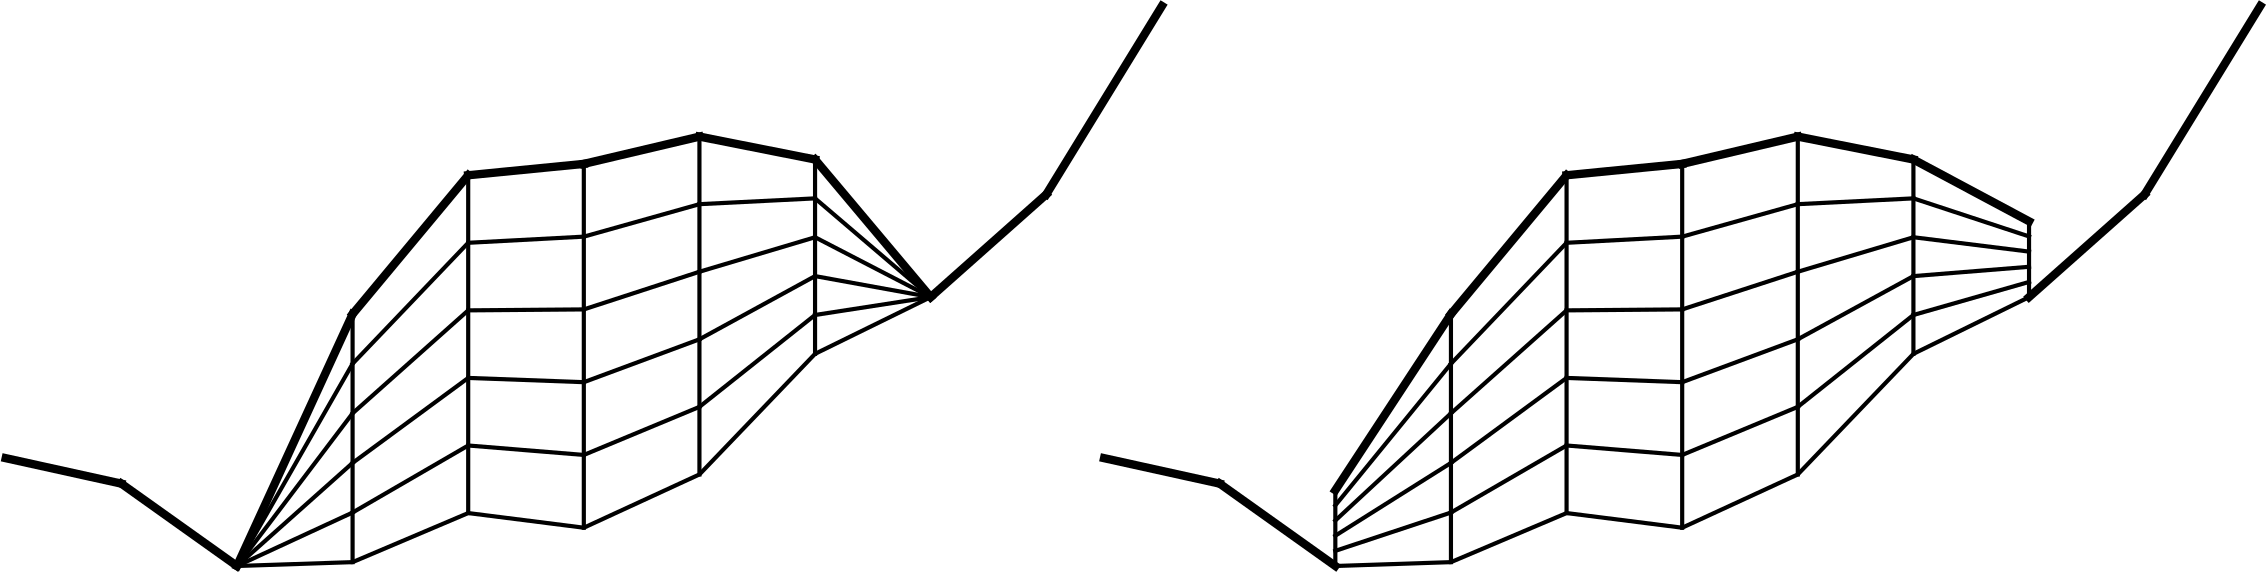
\includegraphics[width=\textwidth]{genfigs/extruded.pdf}
\end{center}
\caption{A sketch of the mass-perturbation approximation in equations \eqref{eq:systemmassanalogy} and \eqref{eq:massanalogy}.}
\label{fig:massanalogy}
\end{figure}

FIXME Pseudocode \ref{pc:pnj} for PNJ with bump approximation

\begin{pcode}[ht]
\begin{pseudo*}
\pr{pnj}(s^h,b^h,\id{omega}=1.0)\text{:} \\+
    \ct{check admissibility: $s^h \ge b^h$} \\
    evaluate $\{\rho_i(s^h; 0)\}_{i=0}^{m-1}$  \qquad\qquad \ct{and save the final Newton step linear system} \\
    for $i = 0,\dots,m-1$ \\+
        $\alpha_i = (A^{-1})_{ii}$  \qquad\qquad \ct{FIXME: give correct Jacobian diagonal entry} \\
        if $\alpha_i > 0$ \\+
            $c_i = - \rho_i(s^h; 0) / \alpha_i$ \\--
    for $i = 0,\dots,m-1$ \\+
        if $\alpha_i > 0$ \\+
            $(s^h)_i \gets \max\{(s^h)_i + \id{omega}\,c_i, (b^h)_i\}$ \\-
        else \\+
            $(s^h)_i \gets \beta_i$ \qquad\qquad \ct{non-elliptic case}
\end{pseudo*}
\caption{Projected nonlinear Jacobi smoother using a bump approximation for the Jacobian diagonal entry $\alpha_i$.  Problem \eqref{eq:glenstokesweak} is solved only once per application of \pr{pnj}, but additional linear algebra is needed to compute $\alpha_i$.}
\label{pc:pnj}
\end{pcode}

We finish this section with some observations which are supported by the results reported in Section \ref{sec:results}.  Constructing an efficient smoother is the most difficult part of building an effective multilevel scheme for numerically solving the SIGP.  In the time-stepping approach to steady state, used by almost all existing models, the difficulty is reflected in the nontrivial determination of a valid conditionally-stable time step criterion for the evolving geometry model.  Here the concern is associated to the ``ellipticity'' of the coupled equations for the SIGP, reflected in whether the diagonal Jacobian entry $\alpha_i$, used in the above pointwise smoothers, is indeed positive.

In fact, suppose $s^h$ gives the $P_1$ geometry of the ice which solves the discrete SIGP.  For each icy node $i$ in $\Omega$, i.e.~such that $(s^h)_i>(b^h)_i$, one can see that $\alpha_i>0$ if and only if the addition of a thin (e.g.~one meter) layer of ice to surface of the ice, covering the vicinity of node $i$ (e.g.~the support of $\psi_i$) will cause a dynamical response in which the surface goes down.  One can show this is so for the SIA theory \cite{JouvetBueler2012}, but, even for nonsliding ice, we know of no proof that the Glen-Stokes SIGP always gives $\alpha_i>0$ at icy locations.  It follows that pointwise smoothers like \pr{pngs\_slow} and \pr{pnj} are inherently fragile across a full range of glacier geometries.


\section{Multilevel constraint decomposition} \label{sec:mcdstokes}

In this section we propose a multilevel scheme for solving the discrete SIGP weak form \eqref{eq:fesigpweakform} using iterated V-cycles of a new method descended from the multilevel constraint decomposition (MCD) method of \cite{Tai2003} (see also \cite{GraeserKornhuber2009}).  Our nonlinear variant of MCD, denoted MCDN, uses a full approximation scheme (FAS) multigrid \cite{Trottenbergetal2001} approach which transfers both the current residual and an approximation of the solution down to coarser levels.

We need notation for multiple mesh levels.  Suppose $\mathcal{T}^0$ is a fixed triangulation of $\Omega$, the coarse level.  Suppose $\{\mathcal{T}^j\}_{j=0}^J$ are standard uniform refinements of $\mathcal{T}^0$ by edge bisection so that each $T \in \mathcal{T}^j$ becomes four similar triangles in $\mathcal{T}^{j+1}$ \cite{Braess2007}.  (If $d=1$ this becomes simple halving of each interval.)  We seek a solution of \eqref{eq:fesigpweakform} on the fine level $\mathcal{T}^J$.  Let $\mathcal{V}^j$ be the $P_1$ FE space on $\mathcal{T}^j$ and $m_j$ be the number of nodes in, and dimension of, $\mathcal{V}^j$.

Suppose $b^J \in \mathcal{V}^J$ denotes the fine-level bed topography.  On this fine level the admissible surface elevations form a closed and convex set $\mathcal{L}^J = \{r^J \ge b^J, r^J|_{\partial\Omega} = b^J|_{\partial\Omega}\} \subset \mathcal{V}^J$.  However, instead of defining such admissible sets on each level, presumably via coarse interpolants of $b^J$, we follow \cite{GraeserKornhuber2009} in creating a multilevel decomposition starting from the defect obstacle for the current fine-level iterate $s^J$.  That is, suppose FIXME

Before describing the MCDN approach we should first be clear about when an iteration has converged.  For a discrete obstacle $\varphi^j \in \mathcal{V}^j$, an admissible current iterate $s^j\in \{r^j \ge \varphi^j\} \subset \mathcal{V}^j$, and a residual vector $F^j \in (\mathcal{V}^j)'$ let
\begin{equation}
\vertiii{F^j}_{(s^j,\varphi^j)} = \left(\sum_{s_i > \varphi_i} |F[\psi_i]|^2 + \sum_{s_i = \varphi_i} |\min\{F[\psi_i],0\}|^2\right)^{1/2} \label{eq:cpnorm}
\end{equation}
be the ``CP residual norm'' associated to the finite-dimensional complementarity problem (CP) $s^j \ge \varphi^j$, $F(s^j) \ge 0$, and $(s^j-\varphi^j) F(s^j) = 0$.  Note $s^j \in \mathcal{V}^j$ solves this CP if and only if $s^j$ is admissible and $\vertiii{F(s^j)}_{(s^j,\varphi^j)}=0$.  As shown in Pseudocode \ref{pc:mcdn-solver} we will iterate MCDN V-cycles until the CP residual norm is small according to either an absolute or a relative tolerance.

\begin{pcode}[ht]
\begin{pseudo*}
\pr{mcdn-solver}(J,s^J,b^J,\id{atol}=10^{-20},\id{rtol}=10^{-3},\id{cyclemax}=100)\text{:} \\+
    function $\rho(s)[r] = F^J(s)[r] - \ip{a}{r}$ \qquad\qquad \ct{residual of \eqref{eq:fesigpweakform}} \\
    $\rho_0=\vertiii{\rho(s^J)}_{(s^J,b^J)}$ \\
    for $k=1,\dots,\id{cyclemax}$ \\+
        $\chi^J = b^J - s^J$ \qquad\qquad \ct{fine-level defect obstacle} \\
        $s^J \gets s^J + \pr{mcdn-vcycle}(J,s^J,\chi^J)$ \\
        $\rho_k=\vertiii{\rho(s^J)}_{(s^J,b^J)}$ \\
        if $\rho_k < \id{atol}$ or $\rho_k \le \id{rtol} \, \rho_0$ \\+
            break \\--
\end{pseudo*}
\caption{The SIGP is solved by iterating V-cycles (Pseudocode \ref{pc:mcdn-vcycle}) until the CP residual norm \eqref{eq:cpnorm} is small.}
\label{pc:mcdn-solver}
\end{pcode}

FIXME MCD theory

FIXME nonlinear MCD V-cycle Pseudocode \ref{pc:mcdn-vcycle}

\begin{pcode}[ht]
\begin{pseudo*}
\pr{mcdn-vcycle}(J,w^J,N,\ell^J,\chi^J,\id{down}=1,\id{coarse}=1,\id{up}=0)\text{:} \\+
    $g^J = w^J$ \\
    for $j=J$ downto $j=1$ \\+
      $\chi^{j-1} = \mR \chi^j$ \\
      $\phi^j = \chi^j - P\chi^{j-1}$ \\
      $y^j = 0$ \\
      $\text{\pr{smoother}}^{\text{\id{down}}}(j,g^j,y^j,N^j,\ell^j,\phi^j)$ \qquad \ct{smoothing in $\mathcal{K}^j$} \\
      $F = N^j(g^j+y^j) - \ell^j$ \\
      $g^{j-1} = \iR(g^j + y^j)$ \\
      $\ell^{j-1} = N^{j-1}(g^{j-1}) - R F$ \\-
    $y^0 = 0$ \\
    $\text{\pr{smoother}}^{\text{\id{coarse}}}(0,g^0,y^0,N^0,\ell^0,\chi^0)$ \\
    $z^0 = y^0$ \\
    for $j=1$ to $j=J$ \\+
      $z^j = P z^{j-1} + y^{j}$ \\
      $\text{\pr{smoother}}^{\text{\id{up}}}(j,g^j,z^j,N^j,\ell^j,\chi^j)$ \qquad \ct{smoothing in $\mathcal{D}^j$} \\-
    return $z^J$
\end{pseudo*}
\caption{FIXME Nonlinear MCD V-cycle.}
\label{pc:mcdn-vcycle}
\end{pcode}


\section{Results for steady geometry} \label{sec:results}

FIXME in this paper the Glen-Stokes problem is solved by Newton linearization and (parallel) direct solution of the Newton step equations; Firedrake and PETSc \cite{Balayetal2020,Bueler2021} used to solve this dynamics problem and thereby evaluate the residual $F$; geometric multigrid schemes exist for the  Glen-Stokes problem \cite{IsaacStadlerGhattas2015}; see also \cite{BrownSmithAhmadia2013} and \cite{Tuminaroetal2016} which solve a first-order approximation of the Glen-Stokes ice sheet problem by geometric and algebraic multigrid, respectively

FIXME convergence results; scaling results


\section{Multilevel methods for evolving geometry} \label{sec:evolution}

FIXME time-dependent runs


\section*{Acknowledgments}  Thanks to David Maxwell for suggestions on the formulation and well-posedness of the model.

\small

\bigskip
\bibliography{msg}
\bibliographystyle{siam}

\appendix

\section{Glossary of acronyms} \label{app:glossary}

\renewcommand{\arraystretch}{1.1}
\begin{longtable}{l|l|l}
\toprule
\textbf{Acronym} {\Large$\strut$} & \textbf{Definition} & \textbf{Reference} \\ \hline
CMB & climatic mass balance & Section \ref{sec:stokesgeometry} \\
FAS & full approximation scheme & Section \ref{sec:mcdstokes} \\
FE & finite element & Section \ref{sec:fe} \\
GS & Gauss-Seidel & Section \ref{sec:smoothers} \\
IDO & ice dynamics operator & Section \ref{sec:weakido}, equation \eqref{eq:ido} \\
IIGP & implicit ice geometry problem & Section \ref{sec:evolution} \\
MCD & multilevel constraint decomposition & Section \ref{sec:mcdstokes} \\
MCDN & multilevel constraint decomposition (nonlinear) & Section \ref{sec:mcdstokes}, Pseudocode \ref{pc:mcdn-vcycle} \\
NCP & nonlinear complementarity problem & Section \ref{sec:stokesgeometry} \\
PNJ & projected, nonlinear Jacobi (smoother) & Section \ref{sec:smoothers}, Pseudocode \ref{pc:pnj} \\
SIA & shallow ice approximation & Section \ref{sec:intro} \\
SIGP & steady ice geometry problem & Section \ref{sec:stokesgeometry}, equation \eqref{eq:strongform} \\
SKE & surface kinematical equation & Section \ref{sec:stokesgeometry}, equation \eqref{eq:ske} \\
VI & variational inequality & Section \ref{sec:weakido} \\
WU & work units & Section \ref{sec:mcdstokes} \\ % final \\ required
\bottomrule
\caption{Glossary of acronyms used in this paper.}
\label{tab:acronyms}
\end{longtable}

\end{document}
